% =====================================================================
%  §2 Degenerations of unitary Conformal Field Theories  （原文 p4–p12）
% =====================================================================
\section{酉共形场论的退化}

本节将说明我们的镜像对称图景的物理动机。我们假定读者对共形场论（conformal field
theory，CFT）的基本概念已有一定程度的了解；例如，\cite{Gaw} 的讲义包含了我们所需的
大部分内容。

酉共形场论（unitary conformal field theory，下文简称 CFT）在数学上有严格定义，它由
以下数据描述：

\begin{enumerate}[label=\arabic*)]
\item 一个实数 $c\ge 0$，称为中心荷（central charge）。
\item 一个双分次的预希尔伯特态空间（pre-Hilbert space of states）
  $H=\oplus_{p,q\in\R_{\ge0}}H^{p,q}$，$p-q\in\Z$，使得对每个 $E\in\R_{\ge0}$，
  $\dim(\oplus_{p+q\le E}H^{p,q})$ 有限。等价地说，存在 Lie 群 $\C^*$ 在 $H$ 上的作用，
  使得 $z\in\C^*$ 在 $H^{p,q}$ 上以 $z^p\bar z^q:=(z\bar z)^p\bar z^{q-p}$ 作用。
\item Virasoro 代数与反 Virasoro 代数之积 $\mathit{Vir}\times\overline{\mathit{Vir}}$
  （中心荷同为 $c$）在 $H$ 上的作用，使得空间 $H^{p,q}$ 是生成元 $L_0$（相应地
  $\bar L_0$）的特征空间，特征值为 $p$（相应地 $q$）。
\item 空间 $H$ 还带有一些由算子乘积展开（operator product expansion，OPE）导出的
  附加结构。OPE 由一个线性映射
  \[
    H\otimes H\longrightarrow H\hat\otimes\C\{z,\bar z\}
  \]
  描述。这里 $\C\{z,\bar z\}$ 是形式幂级数
  $f=\sum_{p,q}c_{p,q}z^p\bar z^q$ 的拓扑环，其中 $c_{p,q}\in\C$，$p,q\to+\infty$，
  $p,q\in\R$，$p-q\in\Z$。OPE 满足一列公理，此处不再赘述（见 \cite{Gaw}）。
\end{enumerate}

设 $\phi\in H^{p,q}$。则数 $p+q$ 称为 $\phi$ 的「共形维数」（conformal dimension），
也称「能量」；$p-q$ 称为 $\phi$ 的「自旋」（spin）。注意，由于 $\phi$ 的自旋是整数，
条件 $p+q<1$ 蕴涵 $p=q$。

中心荷 $c$ 可由公式
\[
  \dim\Bigl(\oplus_{p+q\le E}H^{p,q}\Bigr)
  =\exp\Bigl(\sqrt{\tfrac{4}{3}\pi^2cE\,(1+o(1))}\Bigr),
  \qquad E\to+\infty
\]
描述。可以期待，所有可能的中心荷构成 $\Q_{\ge0}\subset\R_{\ge0}$ 的一个可数良序子集。
若 $H^{0,0}$ 是一维向量空间，则相应的 CFT 称为不可约的。一般的 CFT 是不可约 CFT 之和。
平凡 CFT 满足 $H=H^{0,0}=\C$，它是 $c=0$ 的唯一不可约酉 CFT。

\begin{rmk}
本文的几何讨论与 $N=2$ 超共形场论（superconformal field theory，SCFT）有关。上述
数据与公理有相应的 SCFT 版本。特别地，每个 $H^{p,q}$ 是 Hermite 超向量空间；$H$ 上有
Virasoro 代数与反 Virasoro 代数之积的超扩张的作用。在下文讨论模空间时，我们将不区分
CFT 与 SCFT，因为除了一些细节之外，主要结论在两种情形下都成立。
\end{rmk}

\subsection{共形场论的模空间}

对给定的 CFT，可以考察它的对称群（即空间 $H=\oplus_{p,q}H^{p,q}$ 的、保持所有结构的
自同构群）。可以期待，对称群是维数不超过 $\dim H^{1,0}$ 的紧 Lie 群。

固定 $c_0\ge0$ 与 $E_{min}>0$，考虑中心荷 $c\le c_0$ 且
\[
  \min\{p+q>0\mid H^{p,q}\ne0\}\ge E_{min}
\]
的所有不可约 CFT 构成的模空间 $\MM^{E_{min}}_{c\le c_0}$。可以期待
$\MM^{E_{min}}_{c\le c_0}$ 是局部维数有限的紧实解析叠。给定 CFT 的极小泛形变的底空间的
维数不超过 $\dim H^{1,1}$。我们定义
$\MM_{c\le c_0}=\bigcup_{E_{min}>0}\MM^{E_{min}}_{c\le c_0}$。

我们希望通过添入一些边界分支来紧化这个叠，这些边界分支对应于 $E_{min}\to0$ 时理论
的一些渐近描述。紧化后的空间期待是紧叠 $\overline{\MM}_{c\le c_0}$。下文我们不再严格
区分，笼统地用「空间」一词代替「叠」。

\begin{yizhu}[「叠」与「空间」]
这里的模空间是叠（stack）：CFT 带有自同构群，模函子一般不可表示，故模空间除了记录
对象之外还要记录对象之间的自同构。原文紧接着声明「笼统地用『空间』代替『叠』」，
是因为本节只关心底层的粗模空间及其边界分层，不涉及叠的精细结构。
\end{yizhu}

\begin{rmk}
数学上有严格定义的 CFT 基本上只有两类：有理理论（rational theory，RCFT）与格共形场论
（lattice CFT）。本文的讨论对应于 $\sigma$ 模型的情形，而 $\sigma$ 模型不属于这两类。把 $\sigma$ 模型
描述为对应于某些拉格朗日量的路径积分，迄今尚未给出数学上令人满意的构造。下文我们
将说明，可以用 CFT 的退化来谈论 $\sigma$ 模型，这是另一条途径。
\end{rmk}

\subsection{简单坍缩的物理图景}

为了紧化 $\MM_{c\le c_0}$，我们考察 $E_{min}\to0$ 时 CFT 的退化。一个退化由如上双分次
空间的单参数（离散或连续）族 $H_{\eps}$（$\eps\to0$）给出，其中
$(p,q)=(p(\eps),q(\eps))$。这些空间带有 OPE。共形维数在 $\eps\to0$ 时趋于零的那些场
构成的子空间给出一个交换代数
\[
  H^{small}=\oplus_{p(\eps)\ll1}H_{\eps}^{p(\eps),p(\eps)}
\]
（代数结构由 OPE 的首项给出）。$H^{small}$ 的谱 $X$ 期待是紧空间（「带奇点的流形」），
且 $\dim X\le c_0$。由共形不变性与 OPE 可知，$H^{small}$ 的分次（在 $\eps\to0$ 时
重新标度后）由 $X$ 的光滑部分上某个二阶微分算子的特征值给出。该算子的特征值为正，
且在不计一个标量因子的意义下确定。这意味着 $X$ 的光滑部分带有度量 $g_X$，它同样在
不计一个标量因子的意义下确定。OPE 中的其余项给出 $X$ 上的附加微分几何结构。

于是，作为真实图景的一阶近似，我们对 CFT 族的「简单坍缩」作如下描述。族的退化由
$\MM_{c\le c_0}$ 的边界上一点描述，该点是一个三元组
$(X,\R^*_+\cdot g_X,\phi_X)$，其中度量 $g_X$ 在不计正常数因子的意义下确定，而
$\phi_X:X\to\MM_{c\le c_0-\dim X}$ 是一个映射。对这些数据还可以加一些额外条件，例如
度量 $g_X$ 可以满足 Einstein 方程。

\begin{yizhu}[三元组 $(X,\R^*_+\cdot g_X,\phi_X)$ 的含义]
$X$ 是坍缩后剩下的「底空间」；写成 $\R^*_+\cdot g_X$ 是强调度量只确定到正常数倍，
这正是坍缩图景中尺度不可见的体现。映射 $\phi_X$ 则记录每一点上方残余的 CFT，其中心荷
比原理论少了 $\dim X$；下一段把 $H_{\eps}$ 看成 $H^{small}$-模、并把它视为某个无穷维
向量丛 $W\to X$ 的截面空间，说的正是 $\phi_X$ 的来源。
\end{yizhu}

尽管度量的标量因子是任意的，仍应设想 $g_X$ 的曲率「很小」、$g_X$ 的单射半径「很大」。
映射 $\phi_X$ 从上文所述的 CFT 简单坍缩来看是自然出现的。事实上，在 $\eps\to0$ 的
极限下，空间 $H_{\eps}$ 成为 $H^{small}$-模，可以把它看成无穷维向量丛 $W\to X$ 的
截面空间。可以论证，$W$ 的纤维一般地是中心荷不超过 $c_0-\dim X$ 的 CFT 的态空间；
这一点编码在映射 $\phi_X$ 之中。当 $\phi_X(X)$ 中的 CFT 具有非平凡对称群时，还应期待
$X$ 上有某种规范理论。

纯玻色 $\sigma$ 模型对应于 $c_0=c(\eps)=\dim X$、且残余理论（即 $\phi_X$ 的像中的 CFT）全为
平凡的情形。此时目标空间 $X$ 应带有 Ricci 平坦度量。在超对称情形，目标空间 $X$ 是
Calabi--Yau 流形，而残余的 CFT 丛是自由费米子理论丛。

\begin{rmk}
我们期待所有紧 Ricci 平坦流形（度量在不计常数标量因子的意义下）都作为退化 CFT 的
目标空间出现。因此，CFT 模空间紧化的构造应当把 Einstein 流形模空间的紧化作为一个
组成部分包含在内。注意微分几何中有 Gromov 的一个基本结果（见 \cite{G}）：给定维数、
Ricci 曲率有下界的带基点连通完备黎曼流形，其模空间是预紧的。CFT 模空间的紧化与
Gromov 紧化之间有深刻的联系。由某些物理论证似乎可以推出：所有作为 CFT 极限出现的
目标空间都具有非负 Ricci 曲率。
\end{rmk}

\subsection{多重坍缩与边界的结构}

用 Virasoro 算子 $L_0$ 来说，坍缩由 $L_0$ 的特征值集合中一个「以相同速度」趋于零
（当 $E_{min}\to0$ 时）的子集（簇）$S_1$ 描述。坍缩的下一层次由 $L_0$ 特征值的另一个
子集 $S_2$ 描述：$S_2$ 的元素「模去第一次坍缩」趋于零（即速度相同，但比 $S_1$ 的
元素「慢得多」）。可以继续构造退化的塔。由此得到边界分层的层级结构。也就是说，若
还有以 $X$ 为参数的 CFT 的进一步退化，就得到三元组
$(X,\R^*_+\cdot g_X,\phi_X)$ 的空间上的一个纤维丛，其纤维是同类三元组的空间。最终
我们得到边界 $\partial\MM_{c\le c_0}$ 的如下定性几何图景。

边界点由以下数据给出：
\begin{enumerate}[label=\arabic*)]
\item 紧拓扑空间的一个有限映射塔 $p_i:\overline{X}_i\to\overline{X}_{i-1}$，
  $0\le i\le k$，$\overline{X}_0=\{pt\}$。
\item 一列光滑流形 $(X_i,g_{X_i})$，$0\le i\le k$，使得 $X_i$ 是 $\overline{X}_i$ 的
  稠密子空间，$\dim X_i>\dim X_{i-1}$，且 $p_i$ 定义纤维丛 $p_i:X_i\to X_{i-1}$。
\item $p_i$ 限制到 $X_i$ 上所得纤维丛的各纤维上的黎曼度量，使得每条纤维的直径有限。
  特别地，$X_1$ 的直径有限，因为它是映射 $p_1:X_1\to\{pt\}$ 的唯一纤维。
\item 一个映射 $X_k\to\MM_{c\le c_0-\dim X_k}$。
\end{enumerate}

上述数据在群 $(\R^*_+)^k$ 的自然作用（它重新标度纤维上的度量）下视为等同。

还有一些附加数据，例如丛 $p_i:X_i\to X_{i-1}$ 上的非线性联络。数据集应满足一些条件，
例如度量上的微分方程。在一般情形下我们无法把这一部分数据更精确地表述出来；下文将在
$N=2$ SCFT（对应于以 Calabi--Yau 流形为目标空间的 $\sigma$ 模型）的情形做到这一点。

\subsection{例：环面模型}

非超对称的环面模型由所谓的 Narain 格以及一些附加数据描述。确切地说，固定中心荷
$c=n$ 为正整数。物理学家所说的 Narain 格 $\Gamma^{n,n}$ 是秩 $2n$、符号差 $(n,n)$ 的
唯一幺模格，可以描述为配有二次型
\[
  Q(x_1,\dots,x_n,y_1,\dots,y_n)=\sum_i x_iy_i
\]
的 $\Z^{2n}$。环面 CFT 的模空间是
\[
  \MM^{tor}_{c=n}=O(n,n,\Z)\backslash O(n,n,\R)/O(n,\R)\times O(n,\R).
\]
等价地，它是 Grassmann 流形的开部分
$\{V_+\subset\R^{n,n}\mid\dim V_+=n,\ Q|_{V_+}>0\}$ 在
$O(n,n,\Z)=\Aut(\Gamma^{n,n},Q)$ 作用下的商。设 $V_-$ 是 $V_+$ 的正交补。则
$\Gamma^{n,n}$ 的每个向量可唯一地写成 $\gamma=\gamma_++\gamma_-$，其中
$\gamma_\pm\in V_\pm$。对相应的 CFT，有
\[
  \sum_{p,q}\dim(H^{p,q})z^p\bar z^q
  =\Big|\prod_{k\ge1}(1-z^k)\Big|^{-2n}
   \sum_{\gamma\in\Gamma^{n,n}}z^{Q(\gamma_+)}\bar z^{-Q(\gamma_-)}.
\]

\begin{yizhu}[Narain 格]
Narain 格 $\Gamma^{n,n}$ 是 $n$ 维环面 $\sigma$ 模型的状态格：配分函数中对
$\gamma\in\Gamma^{n,n}$ 的求和即对动量态与缠绕态的求和，而
$|\prod_{k\ge1}(1-z^k)|^{-2n}$ 是 $2n$ 个自由玻色子的贡献。$\Gamma^{n,n}$ 上的二次型
$Q$ 决定格的符号差 $(n,n)$，故格被它唯一确定。下文 \S2.6 把由这类理论构成的边界
分层称为 T 分层。
\end{yizhu}

我们来试着紧化模空间 $\MM^{tor}_{c=n}$。设有单参数族的环面理论使
$E_{min}(\eps)\to0$。则对 $H_{\eps}$ 中相应的向量有 $p(\eps)=q(\eps)\to0$，这蕴涵
$Q(\gamma(\eps))=0$、$Q(\gamma_+(\eps))\ll1$。容易看出，满足这些条件的向量
$\gamma(\eps)$ 可以相加。于是得到一个秩不超过 $n$ 的（部分）格；在「极大」简单坍缩的
情形，秩等于 $n$。可以看出，相应的边界点给出如下数据：
$(X,\R^*_+\cdot g_X,\phi_X^{triv};B)$，其中 $(X,g_X)$ 是平坦的 $n$ 维环面，
$B\in H^2(X,\R/\Z)$，而 $\phi_X^{triv}$ 是从 $X$ 到 CFT 模空间中平凡理论点的常值
映射。这些数据反过来给出一个环面 CFT，它可以实现为目标空间为 $(X,g_X)$、B 场为 $B$
的 $\sigma$ 模型。$X$ 上残余的 CFT 丛是平凡的。

考虑由族 $(X,\lambda g_X,\phi_X^{triv};B=0)$（$\lambda\in(0,+\infty)$）定义的单参数
CFT 族。该族有两个退化，它们定义 $\partial\MM^{tor}_{c=n}$ 的两个点：当
$\lambda\to+\infty$ 时，得到由 $(X,\R^*_+\cdot g_X,\phi_X^{triv};B=0)$ 定义的环面
CFT；当 $\lambda\to0$ 时，得到 $(X^{\vee},\R^*_+\cdot g_{X^{\vee}},
\phi_X^{triv};B=0)$，其中 $(X^{\vee},g_{X^{\vee}})$ 是对偶平坦环面。

格的进一步退化还可能发生。于是得到格的（从而 CFT 的）紧化模空间的一个分层。紧化中的
点由向量空间的旗 $0=V_0\subset V_1\subset V_2\subset\dots\subset V_k\subset\R^n$
描述；此外还给定一个格 $\Gamma_{i+1}\subset V_{i+1}/V_i$，它在相差一个标量因子的
意义下考虑。这些数据给出环面上的环面丛塔
$X_k\to X_{k-1}\to\dots\to X_1\to\{pt\}$，其纤维为
$(V_{i+1}/V_i)/\Gamma_{i+1}$。若 $V_k\simeq\R^{n-l}$（$l\ge1$），则还有从最后一个
环面丛的全空间 $X_k$ 到中心荷较小的环面理论模空间中点 $[H_k]$ 的映射：
$\phi_n:X_k\to\MM^{tor}_{c=l}$，$\phi_k(X_k)=[H_k]$。

\begin{yizhu}[原文的一处笔误]
原文把上式的映射记为 $\phi_n:X_k\to\MM^{tor}_{c=l}$，而同一句末尾又写作
$\phi_k(X_k)=[H_k]$。由于定义域是全空间 $X_k$，且下标 $n$ 在此处已被维数占用，前者
疑为 $\phi_k$ 之误。译文照原文译出，未作改动。
\end{yizhu}

\subsection{例：$SU(2)$ 的 WZW 模型}

此时我们有一个离散族，$c=\frac{3k}{k+2}$，其中整数 $k\ge1$ 称为级（level）。在
$k\to+\infty$ 的极限下得到带有标准度量的 $X=SU(2)=S^3$。相应的丛是平凡 CFT 的平凡丛
（$c=0$，$H=H^{0,0}=\C$）。对任意紧单连通单群 $G$，类似图景成立。

\subsection{$N=2$ SCFT 的 A 模型与 B 模型作为边界分层}

给定中心荷的 $N=2$ SCFT 的紧化模空间 $\overline{\MM}^{N=2}$ 的边界包含一个开分层，
它由以 Calabi--Yau 流形为目标空间的 $\sigma$ 模型给出。每个分层由四元组
$(X,J_X,\R^*_+\cdot g_X,B)$ 的等价类参数化，其中 $X$ 是紧实流形，$J_X$ 是复结构，
$g_X$ 是 Calabi--Yau 度量，$B\in H^2(X,i\R/\Z)$ 是 B 场。残余的 CFT 丛是自由费米子
理论丛。

由超对称，超共形场论的模空间 $\MM^{N=2}$ 是复流形，局部同构于两个复流形之积。%
\footnote{严格地说，应当排除带有共形维数为 $(2,0)$ 的手征场的模型，例如超凯勒流形上
的 $\sigma$ 模型，见 \cite{AM}。}人们相信这一分解（在相差某些修正的意义下）是整体的。此外，
以 Calabi--Yau 流形为目标空间的 $\sigma$ 模型有两类：A 模型与 B 模型。因此，紧化模空间的
传统图景如下：

\begin{center}
  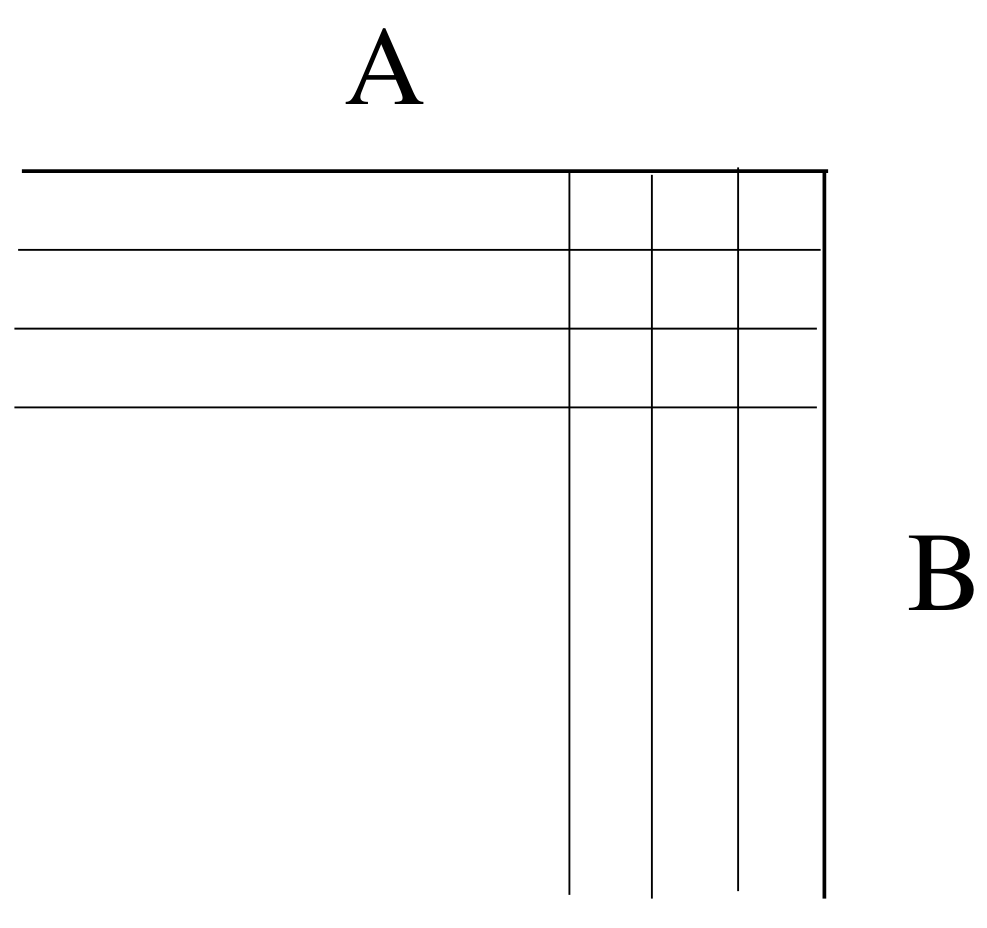
\includegraphics[width=4.18 cm]{figures/fig1_p10_ABstrata}
\end{center}

这里边界由两个开分层（A 分层与 B 分层）以及一个神秘的会合点组成。一般地，这个点
对应于 A 分层的闭包与 B 分层的闭包中一个余维一的子流形。

我们主张这幅图景应当修改：$\partial\overline{\MM}^{N=2}$ 还有另一个开分层（我们称
之为 T 分层），它由环面模型（即与 Narain 格相伴的 CFT）构成，由一个带有不计标量因子
确定的黎曼度量的流形 $Y$ 参数化。这个子簇沿着对应于双坍缩的余维一分层与 A、B 两个
分层都相交。因此，「真正」的图景是传统图景在角点处作实爆破（real blow-up）后得到的：

\begin{center}
  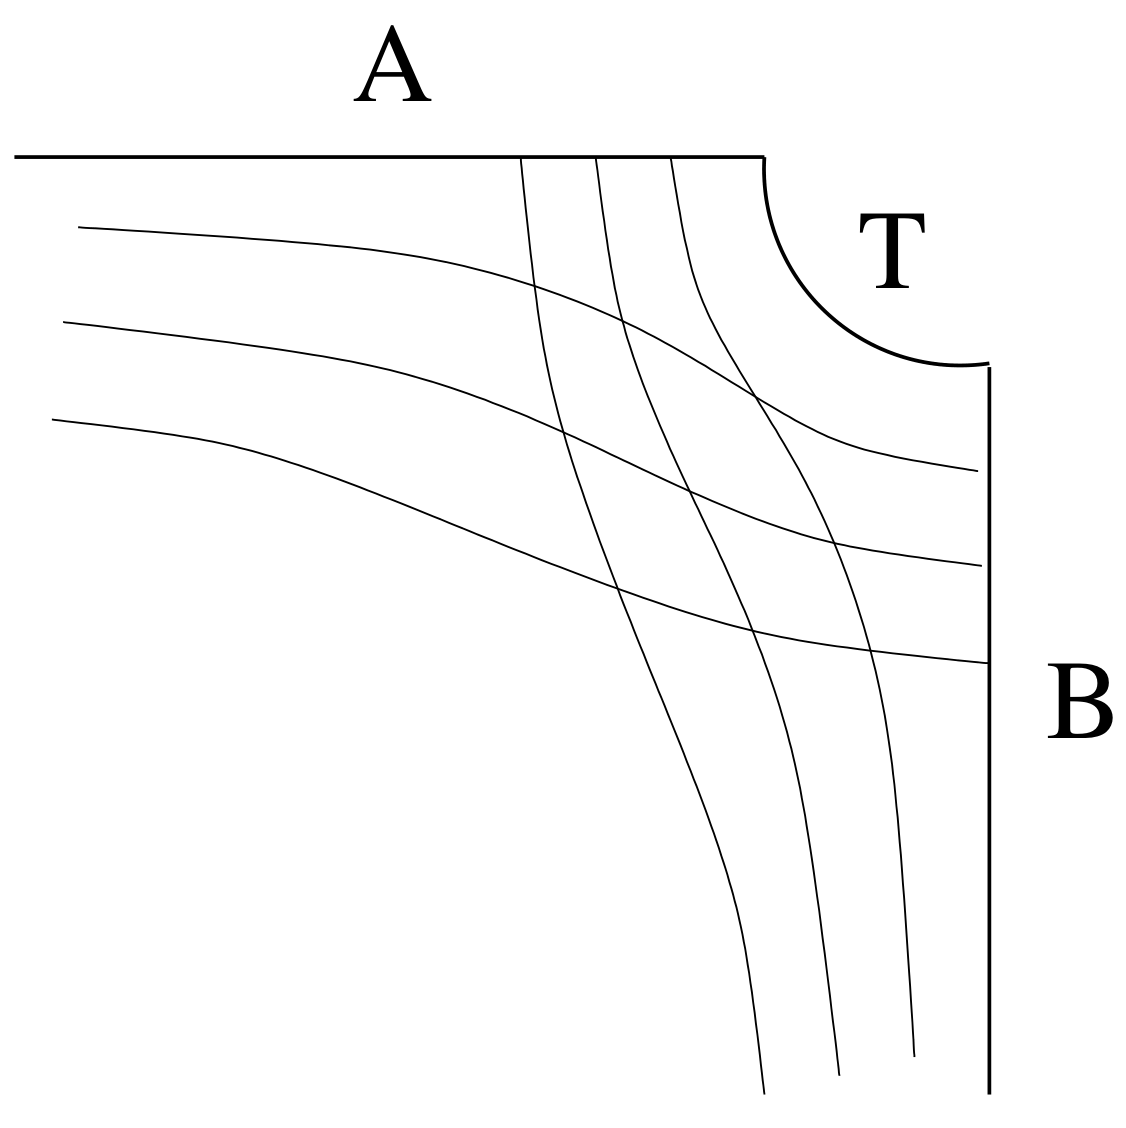
\includegraphics[width=4.77 cm]{figures/fig2_p11_blowup}
\end{center}

\begin{yizhu}[角点处的实爆破]
「实爆破」是指把两条边界相交的角点替换为其方向空间（这里是一段圆弧）：角点被「拉开」，
两个分层不再直接相接，中间多出一段新的边界。原文的图里，这段新边界就是从 A 边界端点
到 B 边界端点的那段圆弧，T 分层正是沿它出现；这也是文中说 T 分层沿余维一的分层与
A、B 二者都相交的意思。
\end{yizhu}

\begin{yizhu}[脚注中的 $(2,0)$ 手征场]
共形维数为 $(2,0)$ 的手征场给出额外的、无质量的自由度，使相应的 $\sigma$ 模型多出原文未计入
的结构（超凯勒目标空间上的 $\sigma$ 模型即是一例），因此必须把这类模型排除在「每层由四元组
参数化」的陈述之外。原文在正文中未展开这一点，只以脚注与文献 \cite{AM} 交代。
\end{yizhu}

\subsection{镜像对称与坍缩}

镜像对称与边界 $\partial\overline{\MM}^{N=2}$ 的两个不同分层（我们称为 A 分层与 B 分层）
的存在有关。作为一个推论，同一批几何对象在不同的分层附近有不同的几何描述。在传统图景中，
可以在对应于 $(X,J_X,\R^*_+\cdot g_X,B)$ 的边界点的小邻域内引入自然坐标。把 $X$ 从
记号中略去，可以说坐标是 $(J,g,B)$（复结构、Calabi--Yau 度量与 B 场）。几何上，
$(g,B)$ 属于凯勒锥在自然映射 $\mathrm{Re}:H^2(X,\C)\to H^2(X,\R)$ 下的原像（更确切
地说，应把 $B$ 看成 $H^2(X,i\R/\Z)$ 的元素）。通常的说法是：考虑复化凯勒锥中一个
开区域，它具有这样的性质——与度量的类 $[g]$ 一起，它还包含射线 $t[g]$，$t\gg1$。
镜像对称给出 $(X,J_X,\R^*_+\cdot g_X,B_X)$ 与
$(X^{\vee},J_{X^{\vee}},\R^*_+\cdot g_{X^{\vee}},B_{X^{\vee}})$ 的邻域之间的一个
等同，使得 $J_X$ 与 $[g_{X^{\vee}}]+iB_{X^{\vee}}$ 互换，反之亦然。

我们可以用另一种方式描述这幅图景。利用复模空间与凯勒模空间的等同，可以取
$([g_X],B_X,[g_{X^{\vee}}],B_{X^{\vee}})$ 作为 A 分层与 B 分层会合点附近的局部
坐标。这个邻域上有加法半群 $\R_{\ge0}\times\R_{\ge0}$ 的作用，它由公式
\[
  ([g_X],B_X,[g_{X^{\vee}}],B_{X^{\vee}})
  \longmapsto
  (e^{t_1}[g_X],B_X,e^{t_2}[g_{X^{\vee}}],B_{X^{\vee}})
\]
显式给出，其中 $(t_1,t_2)\in\R_{\ge0}\times\R_{\ge0}$。当 $t_1\to+\infty$ 时，模空间
中的点趋近 B 分层，在那里度量只确定到正常数倍；第二个半群 $\R_{\ge0}$ 的作用通过
连续性延拓为 B 分层上的非平凡作用。类似地，在 $t_2\to+\infty$ 的极限下，该流把点
收缩到 A 分层。

若如前所述在角点处作实爆破，这幅图景应当修改。此时半群
$\R_{\ge0}\times\R_{\ge0}$ 的作用仍连续延拓到边界上；向 A 分层与 B 分层的收缩带有
相应的同构于 $\R_{\ge0}$ 的半群的非平凡作用。现在，譬如在 A 分层中取一点，则半群流
沿边界把它带到新的分层，即对应于双坍缩的分层。半群 $\R_{\ge0}\times\R_{\ge0}$ 在该
分层上的作用平凡。双坍缩的点同时也是 $\R_{\ge0}\times\R_{\ge0}$ 作用在 T 分层上的
某个一维轨道的极限点。确切地说，元素 $(t_1,t_2)$ 改变由 Narain 格确定的环面的大小，
以系数 $e^{t_1-t_2}$ 重新标度它们。这个流把 T 分层的点带到双坍缩的另一点，后者随即
可以在 B 分层内部移动。整条路径（它是 $\partial\overline{\MM}^{N=2}$ 与
$\R_{\ge0}\times\R_{\ge0}$-轨道的交）通过环面模型的分层把一个 A 模型与相应的 B 模型
连接起来。我们可以把它描绘如下：

\begin{center}
  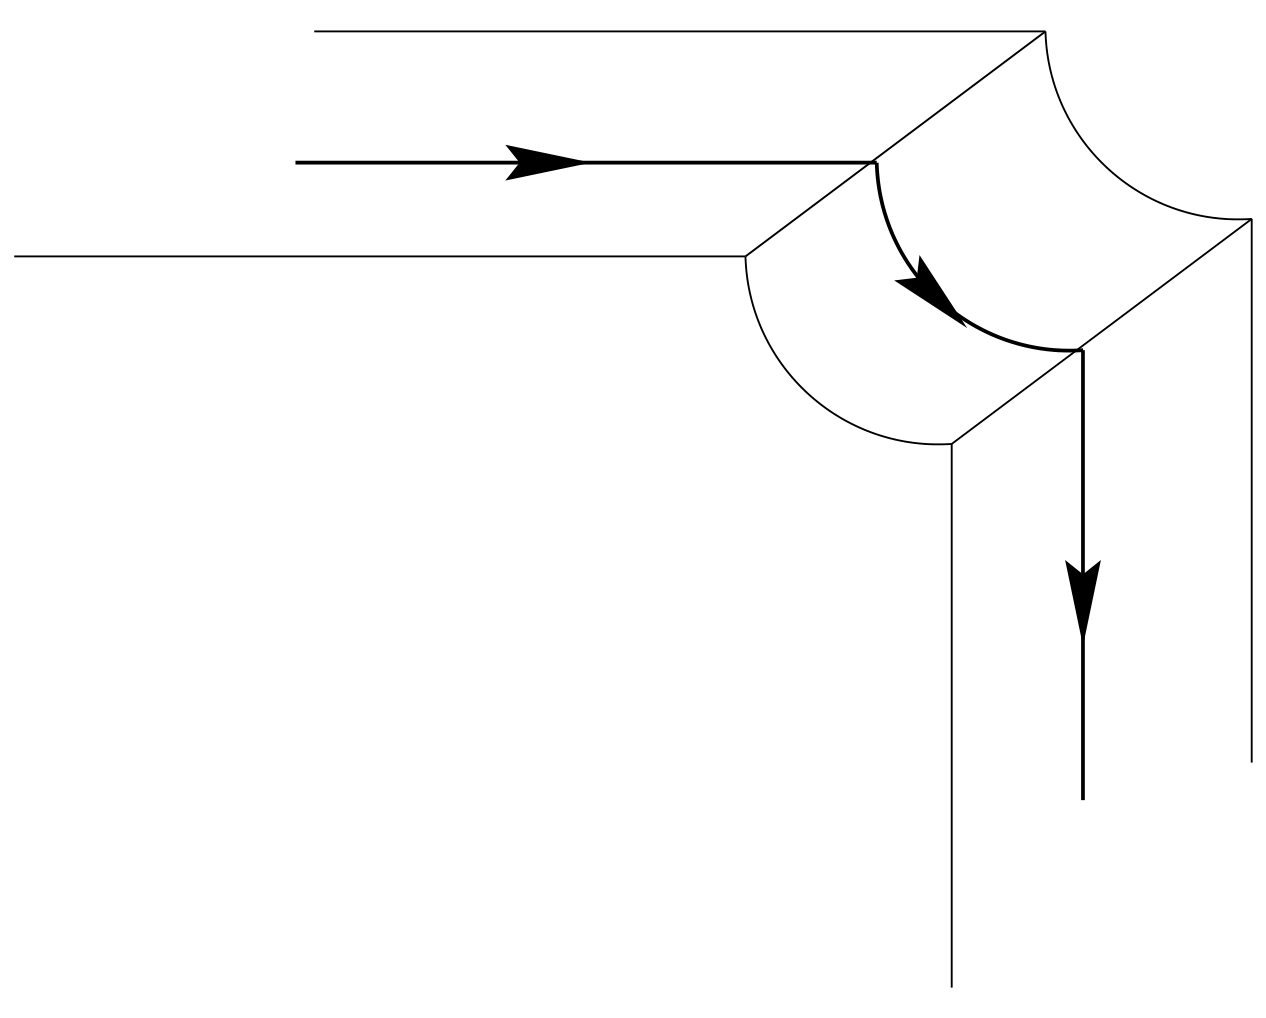
\includegraphics[width=5.36 cm]{figures/fig3_p12_path}
\end{center}

路径的 T 部分（我们称之为 T 路径）连接同一黎曼底空间上的对偶环面纤维化。这就是我们
图景中的镜像对称。

这一描述受到 \cite{SYZ} 的启发。然而读者会注意到，在我们的图景中，镜像对称现象完全
由紧化模空间的\textbf{边界}来解释；为了解释镜像对称现象，并不需要构造完整的 SCFT，
只需处理紧化模空间 $\overline{\MM}^{N=2}$ 边界上的简单环面模型即可。此外，与 \cite{SYZ}
不同，我们的描述不使用超对称圈（D 膜）。

% [原文 p4–p12]
